\chapter{Test scenario and evaluation}
\label{chap:testscenarioandevaluation}

case study, eventuell grosses Beispiel erwaehnen? wenn constraints generiert werden, verlaesst man sich darauf? Hoert man dann auf, selbst mitzudenken? Ist die menge der constraints noch handelbar?

As stated in Sect.~\ref{sec:goals}, appropriate support by a graphical editor is important for the usefulness of the developed visual language. We therefore designed and implemented a prototype of such an editor. The proposed constraint generation heuristics is integrated in this prototype as well and could thus be evaluated. The implementation is a java swing component, making it easy to integrate the visual language into other java applications. An API enables an underlying state machine which also influences the state propositions available for constraint editing. Furthermore a particular model checker can be specified for constraint validation. As a default, the symbolic model checker NuSMV~\cite{springerlink:10.1007/s100090050046,NuSMV2} is used.

Fig.~\ref{fig:editor} shows a snapshot of the editor's environment: All functionality needed for constraint editing is provided in the tool bar on the right. It contains draggable elements for creating all operator and proposition types as well as a trashcan for deleting. Constraints can be composed in the dashboard in the center of the editor by drag\&drop. The tab functionality on the left allows multiple constraints to be managed. Each tab shows a small thumbnail of the constraint and a symbol indicating its validity (a warning shield for ``incomplete'', a green shield for ``valid'', a red cross for ``invalid'' or an animated ring for ``validation in progress.'') The magic wand button within the tab pane triggers the constraint generation.

\begin{figure}[htbp]
  \centering
  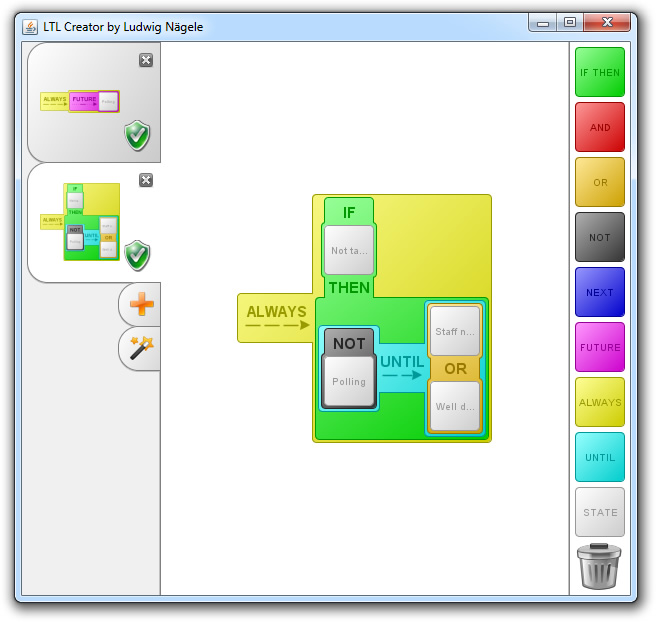
\includegraphics[width=\linewidth]{editor} 
  \caption{Snapshot of the visual editor.}
  \label{fig:editor}
\end{figure}

In order to evaluate the proposed safety functionality the tool was integrated into Robostudio~\cite{robostudio}. This Visual Programming Environment allows the specification of state machine based programs whose behaviour can then be examined by visual constraints. As an example we consider the simplified medication reminder application whose underlying screen-flow is explained in Fig.~\ref{fig:medicationreminder}. Starting from ``Menu'' the user can choose from several services such as blood pressure measurement or entertainment. In the given example these services are simplified to just one state ``additional services'' since we want to focus only on the medication reminder part. In ``Polling'' the database is checked for a pending reminder, and if there is one the medication intake guidance is triggered. The patient can state if he or she has already taken the medication, or decide whether to take it or not. In the latter he or she may give a reason for it and a caregiver is notified about this incident. Otherwise it will result in ``Well done!'' after completing intake.

\begin{figure}[htbp]
  \centering
  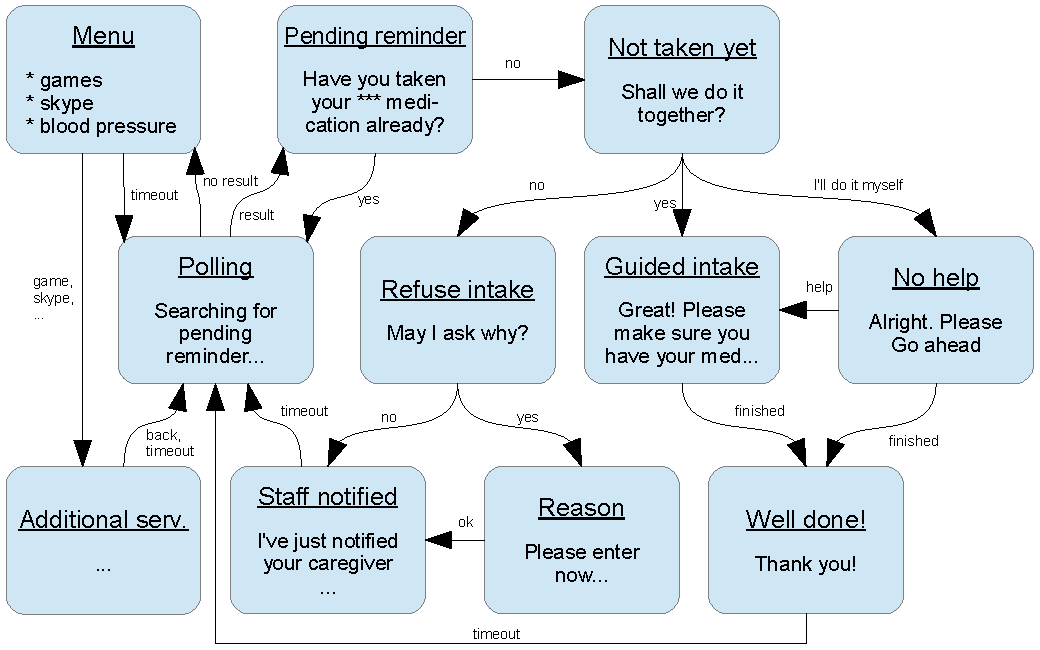
\includegraphics[width=\linewidth]{stm.pdf} %width=0.7\linewidth
  \caption{Simplified screen-flow of the medication reminder application.}
  \label{fig:medicationreminder}
\end{figure}





\section{Operator constraints}

Before we can start creating constraints it might be useful to think about a reasonable term we want to express. Let's take the example ``Whenever there is a pending reminder, medication will be finally taken or caregivers will get notified in case of the patient refusing medication intake.'' given in the requirements in section~\ref{sec:requirements}.

In order to find a corresponding graphical constraint the sentence has to be analyzed just as you read it. Since ``whenever'' is a semantic equivalent to ``always if'' first of all a \emph{ALWAYS} operator gets dragged to the dashboard directly followed by an \emph{IF} as shown in figure~\ref{fig:sampleconstraint}. The condition for this \emph{IF} is that there is a pending reminder, so a state ``Not taken yet'' has to be added to the upper bucket of the \emph{IF} operator.
Whenever the just mentioned condition becomes true, there also has to be true in future: Medication is taken properly or caregivers get notified about refuse. Accordingly a \emph{FUTURE} operator containing an \emph{OR} forms the second part of the \emph{IF} operator. Finally two states 'Well done!' and 'Staff notified' get added to the disjunction. The resulting visual constraint can now automatically be translated to the corresponding LTL formula by the editor:

\begin{equation} \label{eq:sampleconstraint}
  \models \Box (\textnormal{'Not taken yet'} \Rightarrow \Diamond (\textnormal{'Well done!'} \vee \textnormal{'Staff notified'}))
\end{equation}

%This expression can now be translated to the visual form as we just have to break down the formula from the outside to the inside. A surrounding \emph{GLOBALLY} encapsulates an \emph{IF} block since it is the substitution for \emph{IMPLIES}. Its first operator is a proposition \emph{'Not taken yet'} whereas the second parameter has to be a \emph{FOLLOWS} block containing a disjunction of two propositions \emph{'Well done!'} and \emph{'Staff notified'}. The resulting visual constraint is shown in figure~\ref{fig:sampleconstraint}.

\begin{figure}[htbp]
  \centering
  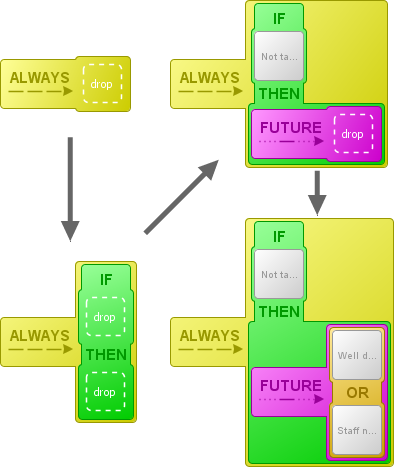
\includegraphics[scale=0.65]{sampleconstraint}
  \caption{Visual constraint creation for LTL formula ~\ref{eq:sampleconstraint}.}
  \label{fig:sampleconstraint}
\end{figure}

After each change in the dashboard, the constraint is automatically recompiled and revalidated by using the underlying model checker. For syntactically invalid constraints, an ``incomplete'' sign is displayed in the respective tab. Otherwise, an animated ring indicates that validation is in pro\-gress and will finally result in either a ``valid'' or ``invalid'' sign.

Due to the optimized performance of NuSMV, even the validation of constraints on huge and complex programs is fast and allows rapid feedback. In addition, the validation itself runs in the background without locking the dashboard. Therefore we avoid waiting times and disruptions during constraint development, which would be likely with conventional model checking where constraint development and constraint validation are alternating processes. Thus we consider our tool an improvement for the user experience.





\subsection{Expressiveness}

Ausdruckss�rke gleich zu LTL, das hei�t, dass lediglich M�glichkeiten nicht ausgedr�ckt werden k�nnen. Zudem gilt eine weitere Einschr�nkung, dass als bedingungen bisher nur Aussagen der Form ``ist in Zustand x'' verwendet werden k�nnen. Da die Validierung der healtbot anwendungen derzeit ausschlie�lich diesen typ braucht, sind andere Bedingungen wie Stringvergleich oder numerische Gleichheit bisher mit der visuellen Sprache nicht m�glich. In Figure~\ref{fig:example_propositions} ist aufgezeigt, wie eine Erweiterung des LTLCreators um weitere Bedingungstypen aussehen k�nnte.


\begin{figure}[htbp]
  \centering
  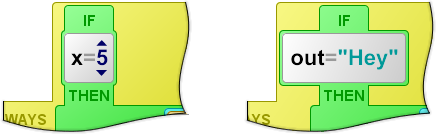
\includegraphics[scale=0.65]{example_propositions}
  \caption{Possible proposition extensions: numeric and string equation.}
  \label{fig:example_propositions}
\end{figure}



\section{Automated Constraint generation}

The automated constraint generation can be triggered by a click on the magic wand button in the tab area. After activation a dashboard is opened in a new tab for each found constraint, and validation is initiated immediately. For the medication reminder application six constraints are found, including \emph{a)} and \emph{b)} shown in Fig.~\ref{fig:generatedconstraints} which match the postulations in the requirements in Sect.~\ref{sec:requirements}.
The constraint used for demonstration in the previous section is also generated, however \emph{b)} forms an intensified restriction of it. 

Constraint \emph{a)} ensures the ``Polling'' state is always eventually visited again. If a pending medication is not already taken, constraint \emph{b)} guarantees intake or staff notification before the next reminders can be read from the database.

We showed that the subgraph approach is working for the medication reminder application, and there was even one more reasonable constraint found by the heuristic: Constraint \emph{c)} ensures that during the medication intake process the program can not switch back to the menu or other services such as entertainment or blood pressure measurement.

%** COMMENT: Possible comment here about the scalability and practicality about constraint generation; do you think it will explode in larger cases? Either way a comment might be useful. **

\begin{figure}[htbp]
  \centering
  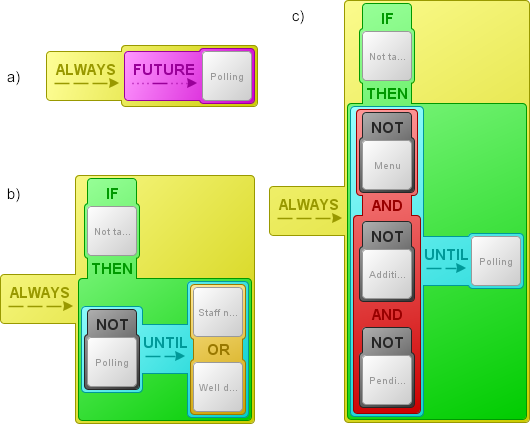
\includegraphics[scale=0.65]{generatedconstraints} %width=0.7\linewidth
  \caption{Automatically generated constraints which match the postulations in the requirements.}
  \label{fig:generatedconstraints}
\end{figure}



%Da der subgraph-finde-algorithmus als brute force algorithmus implementiert wurde kann bei gro�en programmen (ab ca. 1000 Zust�nden und sehr vielen Verzweigungen) der findeprozess teils sehr lange (mehrere Minuten) dauern. Um den warteprozess ertr�glicher zu machen wird w�hrend der findung ein dialog mit dem aktuellen fortschritt und einem abbrechen button angezeigt.
% hat uns die automatische generierung geholfen? Wuhu, wir haben noch einen constraint gefunden, der auch sinn macht



\subsection{Performance}

 (on huge state machines) (brute force algorithm)

\subsection{Scalability}

\subsection{Reasonability of generated constraints}

\section{Reliability}